\documentclass{article}

\usepackage{geometry}
\usepackage{makecell}
\usepackage{array}
\usepackage{multicol}
\usepackage{setspace}
\usepackage{tikz}
\usepackage{multicol}
\usepackage{changepage}
\usepackage{booktabs}
\usepackage{multicol}
\usepackage{wrapfig}
\usepackage{cancel}
\usepackage[explicit]{titlesec}
\usepackage{hyperref}
\usepackage{graphicx}
\usepackage{xcolor}
\usepackage{cprotect}
\usepackage{float}
\newcolumntype{?}{!{\vrule width 1pt}}
\newcommand{\paragraphlb}[1]{\paragraph{#1}\mbox{}\\}
\newcommand{\checkmark}{\tikz\fill[scale=0.4](0,.35) -- (.25,0) -- (1,.7) -- (.25,.15) -- cycle;}
\renewcommand{\contentsname}{Inhaltsverzeichnis:}
\renewcommand\theadalign{tl}
\setstretch{1.10}
\setlength{\parindent}{0pt}

\titleformat{\section}
  {\normalfont\Large\bfseries}{\thesection}{1em}{\hyperlink{sec-\thesection}{#1}
\addtocontents{toc}{\protect\hypertarget{sec-\thesection}{}}}
\titleformat{name=\section,numberless}
  {\normalfont\Large\bfseries}{}{0pt}{#1}

\titleformat{\subsection}
  {\normalfont\large\bfseries}{\thesubsection}{1em}{\hyperlink{subsec-\thesubsection}{#1}
\addtocontents{toc}{\protect\hypertarget{subsec-\thesubsection}{}}}
\titleformat{name=\subsection,numberless}
  {\normalfont\large\bfseries}{\thesubsection}{0pt}{#1}

\hypersetup{
    colorlinks,
    citecolor=black,
    filecolor=black,
    linkcolor=black,
    urlcolor=black
}

\geometry{top=12mm, left=1cm, right=2cm}
\title{\vspace{-1cm}Datenstrukturen und Algorithmen}
\author{Andreas Hofer}

\begin{document}
	\maketitle
	\tableofcontents
	\section{Einführung}
	Datenstrukturen und Algorithmen sind ein essenzieller Bestandteil moderner Systeme, da diese die Geschwindigkeit der meisten Operationen um ein Vielfaches erhöhen. Ob bei Netzwerkrouting, Rendering oder der Kryptographie, Algorithmen finden in allen Facetten des digitalen Bereichs Anwendung. \\
	In der grundlegendsten Form ist ein Algorithmus ein fest beschriebener Weg zur Lösung eines Problems in ihrer allgemeinen Form. Zwei Binärzahlen werden beispielsweise addiert, indem beide Zahlen von rechts nach links verglichen werden und dann anhand der Zahlen diese eine neue Zahl bilden und eventuell eine Zahl in das nächste Register überführt wird. Ein Algorithmus beschreibt also zwar den Lösungsweg für ein Problem aber nicht dessen Implementation. Zusätzlich hat ein Algorithmus stets für eine Eingabe eine eindeutige Ausgabe. \\
	Jedoch muss beachtet werden, dass nicht jedes Problem algorithmisch lösbar (Wie das Halteproblem \hyperref{/../Semester 1/GDI1/GDI.pdf}{halteproblem1}{halteproblem2}{Siehe GDI1}) ist und auch nicht jedes Problem ist praktisch berechenbar (Wie NP-Komplette Probleme [TODO LINK GDI]). \\
	Ein Algorithmus hat einige Eigenschaften:
	\begin{itemize}
		\item{Terminiertheit}
		\begin{itemize}
			\item{Eine Eingabe führt nach einer endlichen Anzahl an Schritten zu einer Ausgabe oder einem Abbruch}
		\end{itemize}
		\item{Finitheit}
		\begin{itemize}
			\item{Es gibt eine endliche Menge an Befehlen}
		\end{itemize}
		\item{Effektivität}
		\begin{itemize}
			\item{Die Auswirkung jedes Befehls innerhalb des Algorithmus ist eindeutig}
		\end{itemize}
		\item{Determiniertheit}
		\begin{itemize}
			\item{Die gleichen Eingaben führen zur gleichen Ausgabe}
		\end{itemize}
		\item{Determinismus}
		\begin{itemize}
			\item{Bei gleichen Eingaben wird auch der selbe Lösungsweg genommen.}
			\item{Ein Algorithmus kann determiniert aber nicht determistisch sein, wenn darin Zufallselemente vorkommen}
		\end{itemize}
	\end{itemize}
	Zusätzlich zur bereits bekannten Zeitkomplexität in der O-Notation (Siehe GDI [TODO GDI Link]) gibt es auch Speicherkomplexität, was beschreibt wie viel zusätzlichen Speicherplatz ein Algorithmus benötigt um das Problem zu lösen. Einen Algorithmus welcher keinen zusätzlichen Speicherplatz benötigt nennt man "In-Place". \\
	\section{Insertion Sort}
	Insertion Sort ist einer der simpelsten Sortieralgorithmen mit jedoch einer relativ hohen Laufzeit. Er funktioniert, indem er stets von links nach rechts ein Array durchläuft und jeweils eine niedrigere mit einer höheren Zahl vertauscht. Diese Zahl wird so lange vertauscht, bis die linke Zahl kleiner ist als die rechte. Danach wird der Zähler nach rechts verschoben und die nächste Zahl verglichen bis man an das Ende des Arrays kommt. \\
	\subsection{Pseudocode}
	Angenommen man hat ein Array [8, 6, 9, 5], dann würde der Prozess in ewta so aussehen: \\
	\begin{tabular}{| l | l | l | l | c | c |}
		\toprule
		i & key & j & A[j] & $A[j]>$key \& $j>0$ & A \\ \midrule
		2 & 6 & 1 & 8 & $8>6\&1>0$ -> True & $[-_1, \textcolor{red}{8}_2, 9_3, 5_4]$ \\
		- & - & 0 & - & - -> False & $[\textcolor{red}{6}_1, 8_2, 9_3, 5_4]$ \\ \hline
		3 & 9 & 2 & 8 & $8>9\&2>0$ -> False & $[6_1, 8_2, 9_3, 5_4]$ \\ \hline
		4 & 5 & 3 & 9 & $9>5\&3>0$ -> True & $[6_1, 8_2, -_3, \textcolor{red}{9}_4]$ \\
		- & - & 2 & 8 & $8>5\&2>0$ -> True & $[6_1, -_2, \textcolor{red}{8}_3, 9_4]$ \\
		- & - & 1 & 6 & $6>5\&1>0$ -> True & $[-_1, \textcolor{red}{6}_2, 8_3, 9_4]$ \\
		- & - & 0 & - & - -> False & $[\textcolor{red}{5}_1, 6_2, 8_3, 8_4]$ \\
		\bottomrule
	\end{tabular}
	\section{Analyse von Algorithmen}
	Die Analyse von Algorithmen ist wichtig um deren Effizienz finden und sie vergleichen zu können. Um diese zu vergleichen wird eine Abstraktion eines Rechners verwendeten, welcher eine spezifische Konfiguration hat. Dieser theoretische Rechner hat folgende Eigenschaften:
	\begin{itemize}
		\item{Es existiert 1 Prozessor, welcher jeweils einen Befehl sequenziell abarbeitet}
		\item{Jede Zahl im Programm passt in eine Speichereinheit}
		\item{Speicherzugriff ist immer gleich schnell}
		\item{Primitive Operationen dauern immer gleich lang. Primitive Operationen sind:}
		\begin{itemize}
			\item{Eine Zuweisung \texttt{a = b}}
			\item{Eine arithmetische Operation wie Addition, Subtraktion, etc \texttt{a + b}}
			\item{Vergleichsoperatoren wie größer, kleiner oder gleich \texttt{a > b}}
			\item{Befehle zur Ablaufsteuerung wie \texttt{if}, \texttt{else} oder \texttt{while} \texttt{if (a == b)}}
		\end{itemize}
	\end{itemize}
	\subsection{Laufzeitberechnung}
	\subsubsection{Sequenz}
	Die Laufzeit einer Sequenz ohne Schleifen wird anhand ihrer Aktionen summiert. Man kann eine arithmetische Operation mit Zuweisung als eine oder zwei Aktionen sehen.
	\begin{figure}[H]
	\centering
	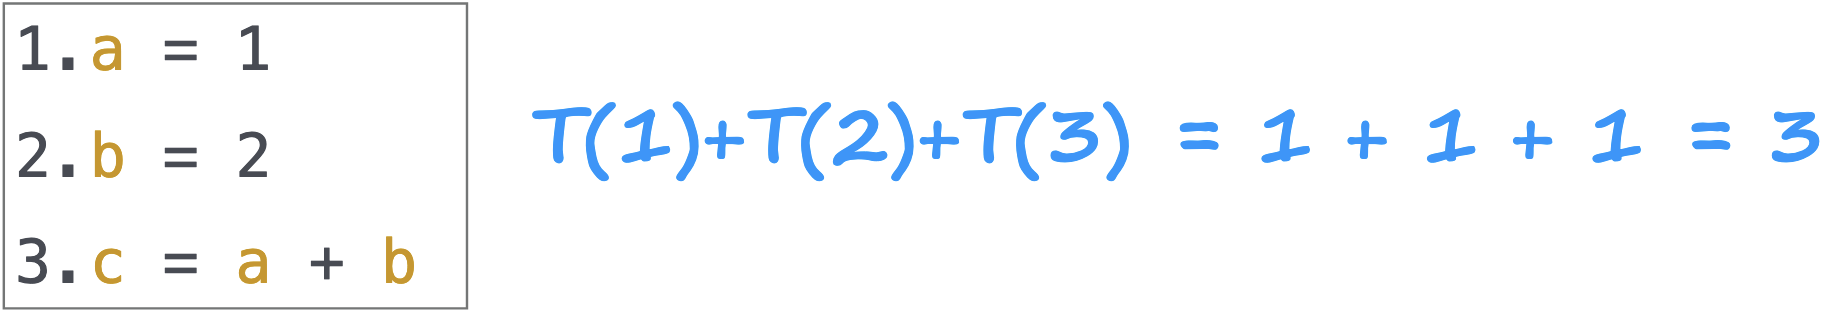
\includegraphics[width=0.48\textwidth]{Bilder/sequence.png}
	\caption{Summierung einer Sequenz an Befehlen}
	\end{figure}
	\subsubsection{Schleifen}
	Bei einer Schleife wird die Menge an Sequenzen mit der Anzahl an Schleifendurchläufen multipliziert. Man muss beachten, dass ein Programm eine Schleife immer noch ein Mal evaluiert, before sie beendet wird, weshalb bei einer Schleife mit 2 Durchläufen die Schleife 3 Mal evaluiert wird (Ein Mal am Anfang, ein Mal nach der Erhöhung und ein Mal am Ende).
	\begin{figure}[H]
	\centering
	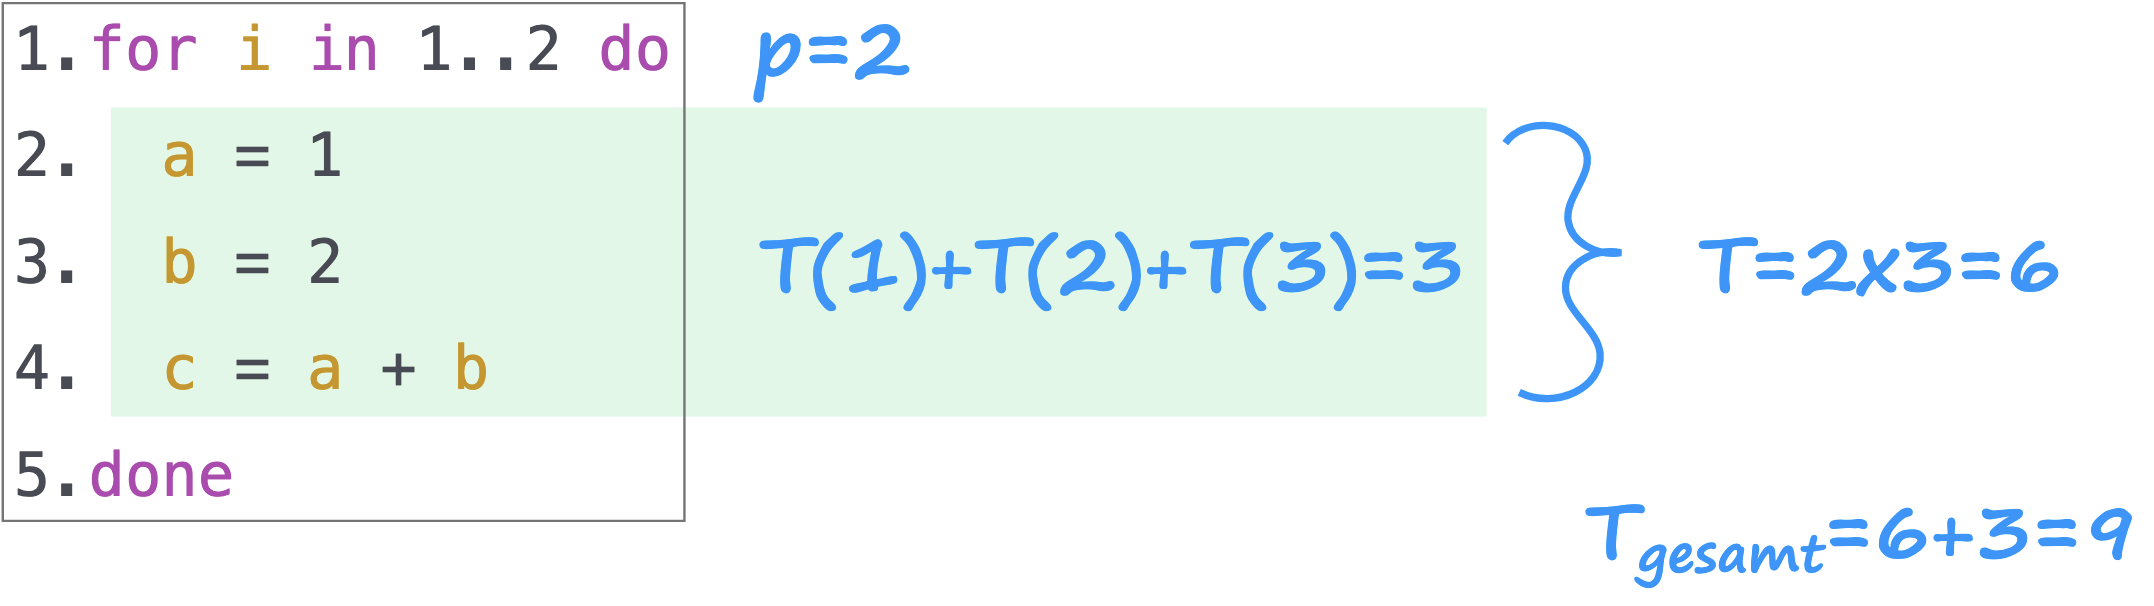
\includegraphics[width=0.48\textwidth]{Bilder/loop.png}
	\caption{Summierung einer Sequenz an Befehlen}
	\end{figure}
	\subsubsection{Verschachtelte Schleifen}
	Wenn Schleifen verschachtelt werden, erhöht sich die Anzahl an Schritten um ein vielfaches. Da eine Schleife mit 5 Ausführungen, welche in einer anderen Schleife mit 10 Ausführungen sitzt, bei jedem der 10 Durchläufe 5 Mal durchlaufen wird muss man die Schritte einer Schleife mit der äußeren Schleife multiplizieren um die Anzahl der Schritte zu erhalten. Also muss man die Schritte in einer Schleife mit der Anzahl an Wiederholungen multiplizieren und danach wiederum mit der Anzahl an Wiederholungen der äußeren Schleife.
	\begin{figure}[H]
	\centering
	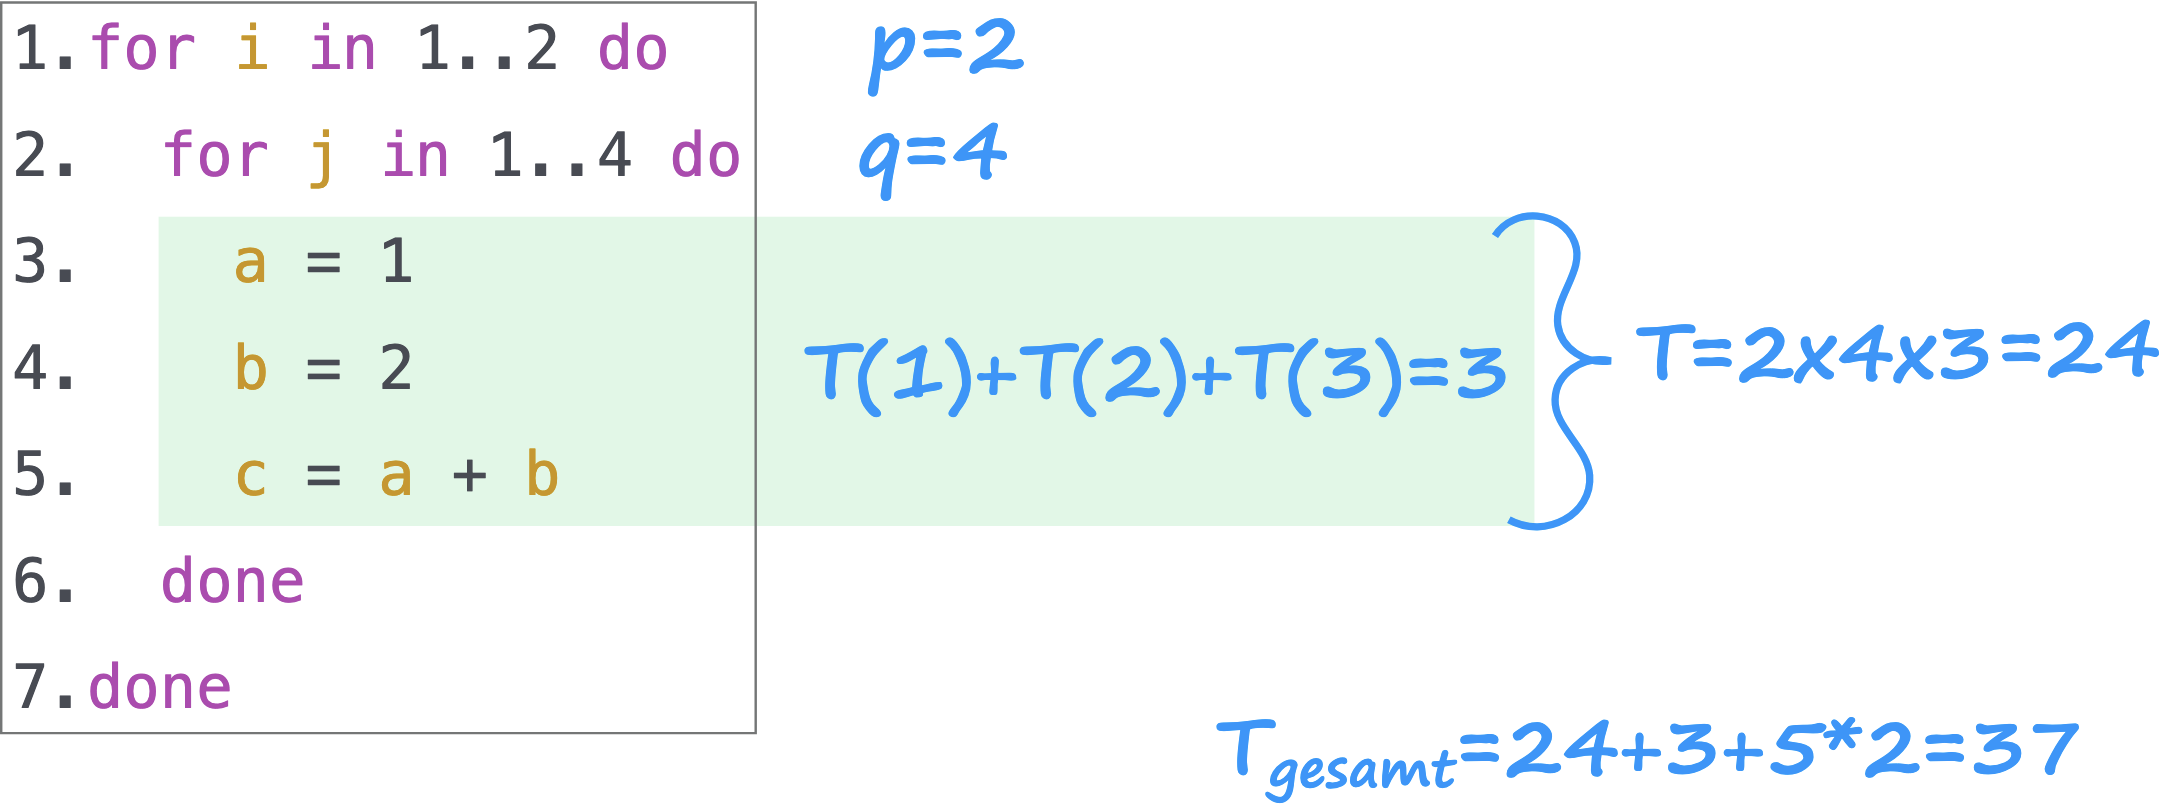
\includegraphics[scale=0.20]{Bilder/nested.png}
	\caption{Laufzeit einer verschachtelten Schleife}
	\end{figure}
	\subsection{Best Case}
	Der Best Case tritt auf, wenn der Algorithmus die geringstmögliche Anzahl an Schritte abhängig von der Eingabe durchläuft. Bei dem Insertion Sort tritt das auf, wenn das Array bereits sortiert ist. \\
	Da trotzdem das Array ein Mal durchlaufen werden muss um dessen Sortiertheit zu überprüfen, ist die Laufzeit n-1 ($\sum_{i=2}^{n}t_i$ => $\sum_{i=2}^{n}1$ => (n-1)) \\
	$T(n)=c_1n+c_2(n-1)+c_3(n-1)+c_4(\sum_{i=2}^{n}t_i)+\cancel{c_5*\sum_{i=2}^{n}(t_i-1)}\cancel{+c_6*\sum_{i=2}^{n}(t_i-1)}+c_7(n-1)$ \\
	$c_1n+c_2(n-1)+c_3(n-1)+c_4(n-1)+c_7(n-1)=(c_1+c_2+c_3+c_4+c_7)n-(c_2+c_3+c_4+c_7)=c_x*n-c_y$ \texttt{Da es sich um einen linearen (cx*n) und einen konstanten (cy) Faktor handelt, dominiert der lineare und es handelt sich deshalb um eine Komplexität von O(n)}
	\subsection{Worst Case}
	Der Worst Case ist das Gegenteil des Best Case und gibt die Laufzeit des Algorithmus an, wenn er die höchstmögliche Arbeit volrichten muss um zum Ergebnis zu bekommen. Das geschieht im Insertion wenn das Array verkehrt sortiert ist, da dadurch jedes Element an das andere Ende des Arrays verschoben werden muss. In diesem Fall hat Insertion Sort eine Laufzeit von $n^2$. \\
	\subsection{Average Case}
	Der Average Case versucht die mittlere Performance eines Algorithmus zu berechnen. In den meisten Fällen ist der Average Case nur unmerklich besser als der Worst Case. Da man die durchschnittliche Verteilung der Inputarrays kennen muss, ist die Berechnung des Average Case relativ aufwändig und normalerweise nur relevant wenn der Worst Case sehr selten eintrifft.
	\section{Landau Notation}
	Wie bereits in Grundlagen der Informatik besprochen, beschreibt die Landau-Notation (O-Notation) die geringste obere Schranke eines Algorithmus. Zur Bestimmung der Laufzeit muss man so stets immer den variablen Teil der Laufzeit mit der höchsten Notation nehmen und diesen als dessen O-Notation angeben. Beispiele sind: \\
	$f(n)=3n^2+n\in O(n^2)$ \\
	$f(n)=5^n+n^2-5\in O(5^n)$ \\
	$f(n)=2\log(5n)n^2+4(\log(n))\in O(log(n)n^2)$ \\
	$f(n)=-2n^2+50n-4\in O(n)$ \texttt{-> Nur ein theoretisches Beispiel. Ein Teil eines Algorithmus kann keine negative Laufzeit haben.} \\
	\subsection{Zugehörigkeit}
	Man kann diese Zugehörigkeit des Grenzwerts jedoch auch direkt berechnen indem man den Limes verwendet: $\lim_{n\to\infty}\frac{f(n)}{g(n)}=K, 0\leq K\leq \infty$ \\
	Wenn man also zwei Funktionen vergleicht kann man diese mittels des limes gegenüberstellen um den schneller ansteigenden zu bestimmen: \\
	$f(n)=42, g(h)=n*\pi, f(n)\in O(g(n))?$ \texttt{Ist f(n) Teil der oberen Schranke?} \\
	$\lim_{n\to\infty}\frac{42}{n*\pi}=0=K$ \texttt{->} $0\leq K < \infty$ \texttt{42 ist also Teil der Schranke} \\
	\subsection{Untere Schranke}
	Während man die obere Schranke die O-Notation nennt, ist die untere Schranke die $\Omega$-Notation. Die Definition ist die selbe, außer, dass die Funktion f(n) stets kleiner oder gleich sein muss als größer. Die Berechnung des Grenzwerts ist ebenfalls der selbe, nur die Einschränkung ist anders, sodass K größer als 0 und kleiner gleich unendlich sein muss: $0 < K \leq \infty$.
	\subsubsection{Berechnung:}
	$2n^2-3n+5\in \Omega(n)?, 0<K\leq\infty$ \\
	$\lim_{n\to\infty}\frac{2n^2-3n+5}{n}=\lim_{n\to\infty}\frac{2n^2}{n}-\lim_{n\to\infty}\frac{3\cancel{n}}{\cancel{n}}+\lim_{n\to\infty}\frac{5}{n}=\infty-3+0=\infty=K$ \texttt{-> 2$n^2$-3n+5 hat Omega(n) als untere Schranke}
	\subsection{Exakte Schranke}
	Zusätzlich existiert noch die Exakte Schranke, auch $\Theta$-Schranke genannt. Während die vorherigen Schranken die obere und untere Grenze suchen, bezeichnet die exakte Schranke die Fläche dazwischen. So muss f(n) stets zwischen der oberen und unteren Schranke existieren. Die Berechnung des Grenzwerts ist wiederum der selbe mit einem anderen Grenzwert, welcher strikt zwischen 0 und unendlich sein muss (Ohne die Erlaubnis gleich wie eine der beiden Seiten zu sein): $0 < K <\infty$
	\subsubsection{Berechnung:}
	$2^n+n^2\in\Theta{2^n}?, 0<K<\infty$ \\ 
	$\lim_{n\to\infty}\frac{2^n+n^2}{2^n}=\lim_{n\to\infty}\cancel{\frac{2^n}{2^n}}+\lim_{n\to\infty}\frac{n^2}{2^n}=1+0+1$
	\section{Datenstrukturen}
	Eine Datenstruktur ist eine Kollektion an Daten, welche geordnet abgespeichert werden. Da solche Datenstrukturen stets wiederum auf Algorithmen beruhen um Daten einzufügen, zu finden und wieder zu löschen, haben auch diese eine Laufzeit. Dabei bieten gewisse Strukturen bessere einfüge-, such- oder Löschzeiten. Eine Datenstruktur besteht deshalb stets aus den gespeicherten Daten sowie dessen Operationen. DS bieten auch oft weitere Operationen wie das i-te Element finden, die Anzahl der Elemente angeben oder den Nachfolger eines Elements zu finden. \\
	\subsection{Elementare Datenstrukturen}
	Es gibt vier elementare Datenstrukturen: Das Array (Lineares Feld), Linked List(Verkettete Liste), Stack (Keller- oder Stapelspeicher) und Queue (Warteschlange). Es gibt jedoch auch kombinierte Datenstrukturen wie zum Beispiel ein Array aus verketteten Listen. Also gibt es viele Arrays, welche jeweils auf das nächste Array zeigen. Diesen Vorgang nennt man auch nesting.
	\subsubsection{Array}
	Ein Array ist in der Lage mehrere Elemente des gleichen Basistyps abzuspeichern. Zugriff auf einzelne Elemente ist mittels des Index möglich. Das Array ist eine statische Datenstruktur, dessen Größe kann also nur ein Mal definiert werden und muss erneut generiert werden um dessen Größe zu erhöhen. Anders als andere Datenstrukture stehen die Daten eines Arrays stets nebeneinander. \\
	Die Zugriffszeiten für ein Array sind: \\
	\begin{tabular}{| l | l | l |}
		\toprule
		Operation & Laufzeit & Erklärung \\ \midrule
		Zugriff auf i-tes Element & O(1) & Da alle Elemente nebeneinander liegen können diese sofort angesprochen werden \\ \hline
		Suchen & O(n) & Da das Array linear iteriert werden muss um einen Wert zu finden. \\ \hline
		Einfügen/Löschen & O(n) & Da man das Array eventuell neu generieren muss. \\ \hline
		Speicherbedarf & O(n) & Jedes Element muss genau ein Mal abgespeichert werden.\\
		\bottomrule
	\end{tabular} \\
	Arrays finden Anwendung wenn eine Liste oder eine Matrize verwendet werden soll. Es ist besonders effizient, wenn man im Vorhinein weiß, wie groß das Array sein muss. Falls man einen Graphen oder ein zweidimensionales Array abbilden will, ist es auch praktisch ein Array zu verwenden. \\
	In Java kann man ein primitives Array mit eckigen Klammern generieren \texttt{int[] -> Generiert ein Array aus Integerwerten.}. Zusätzlich existieren zwei auf Arrays basierenden Collections: Die ArrayList und den Vector. Die ArrayList ist eine dynamische Version eines Arrays, welches neuen Speicher allokiert falls nötig, ohne das dies explizit angegeben werden muss. Vector ist eine ältere Version der ArrayList, welche thread-safe ist, also bei multithreading keine race-condition auslösen kann. \\
	\subsubsection{Linked List}
	Eine Linked List ist eine dynamische Datenstruktur in der jedes Element eine Referenz auf das nächste Element besitzt. Aus diesem Grund müssen die Daten nicht nebeneinander abgespeichert werden, sondern werden über die Pointer gefunden. Dadurch besteht auch keine Garantier, dass folgende Daten auch nebeneinander im Speicher liegen. \\
	Es gibt zwei Arten von Linked Lists: Single-Linked (Einfach verkettete) und Double-Linked (Dopplet-verkettete) Lists. Einfach verkettet Listen haben die Referenz nur in eine Richtung, wodurch man nicht zurückgehen kann. \\
	Die Zugriffszeiten für eine Linked List sind: \\
	\begin{tabular}{| l | l | l |}
		\toprule
		Operation & Laufzeit & Erklärung \\ \midrule
		Zugriff auf i-tes Element & O(n) & Da Pointer durchlaufen werden müssen um das Element zu finden. \\ \hline
		Suchen & O(n) & Da man wieder über die Pointer Elemente suchen muss. \\ \hline
		Einfügen/Löschen des Kopfes & O(n) & Da man das Element nur am Anfang einfügen muss \\ \hline
		Speicherbedarf & O(n) & Jedes Element benötigt zwar Pointer, ist jedoch trotzdem linear.\\
		\bottomrule
	\end{tabular} \\
	Double-Linked Lists besitzen ihre Referenz in beide Richtungen, wodurch man entweder nach vorne oder nach hinten gehen kann. Dadurch besitzt die Liste einen Head und einen Tail (Am Anfang und am Ende), wodurch an beide Enden ein Element angefügt werden kann. Dabei muss man jedoch beachten, dass die Pointer stets die richtigen Elemente als Ziel besitzen. \\
	Eine spezielle Art der Linked-List ist die Circular-List, in welche das letzte Element wiederum auf das erste zeigt, wodurch sie kein Ende besitzt. \\
	Eine Linked List ist sehr effektiv, wenn man nicht weiß, wie viele Elemente man haben wird, da dynamisch weitere hinzugefügt werden können. Bei der dynamischen Speicherverwaltung ist es auch nützlich, da man so die Menge an leeren und besetzten Elementen stets anpassen kann. \\
	In Java existiert eine LinkedList collection, welche eine Double-Linked List implementiert.
	\subsubsection{Stacks}
	Ein Stack (Auf Deutsch Stapel) ist eine dynamische Datenstruktur, bei welcher nur das oberste Element manipuliert werden kann. So kann man nur ganz oben ein Element hinzufügen (Push) und nur das oberste Element jeweils entfernen (Pop). Zusätzlich kann man mittels \texttt{peek} auch den Wert des obersten Elements auslesen ohne es zu entfernen. Dieses Prinzip nennt man auch LIFO, Last-In First-Out. \\
	Ein Weg einen solchen Stack zu implementieren ist mit einem Arrax, welches danach die Elemente sequentiell abspeichert. Dabei muss man jedoch beachten, dass ein Array stets eine statische Größe hat, ein Stack jedoch eigentlich eine dynamische Datenstruktur sein sollte. Nun könnte man jedes Mal, wenn die Maximalgröße erreicht wurde, die Größe des Arrays um 1 erhöhen, das ist jedoch eine sehr ineffiziente Operation da Arrays mit O(n) verschoben werden. Ein besserer Weg dies umzusetzen ist das sogenannte \texttt{Repeated Doubling}, wobei jedes Mal, wenn man die Maximalgröße erreicht hat, das Array in seiner Größe verdoppelt, wodurch das Array stets zwischen 50 und 75\% gefüllt ist. \\
	Ein besserer Weg zur Implementation ist die Linked List, da hierbei Elemente dynamisch aneinandergereiht werden. Und da man stets nur das erste Element braucht, ist auch die schlechtere Suchzeit der Linked List nicht relevant. \\
	Anwendungen des LIFO Prinzips wird für die Evaluierung von Semantik bei Programmiersprachen angewandt. Ebenfalls kann man Undo/Redo Operationen bei Programmen mittels Stack realisieren, da man so die letzten Operationen einfach auf den Stack legt. Um diese zurückgesetzten Operationen wieder zu revidieren kann man einen zweiten Stack machen, welcher Undo Operationen speichert. \\
	Bei einem Programmablauf gibt es auch den Call Stack, welcher die Reihenfolge von Methodenaufrufen abspeichert. \\
	Die Zugriffszeiten für einen Stack sind sind: \\
	\begin{tabular}{| l | l | l |}
		\toprule
		Operation & Laufzeit & Erklärung \\ \midrule
		Zugriff auf i-tes Element & O(n) [O($n^2$)] & \makecell[l]{Ein Element zu finden ist O(n) man muss jedoch eventuell Elemente \\ zurücklegen,  weshalb es O($n^2$) sein könnte} \\ \hline
		Suchen & O(n) [O($n^2$)] & Gleich wie bei dem Zugriff. Mit O(n) oder O($n^2$) \\ \hline
		Einfügen/Löschen des Kopfes & O(1) [O(n)] & Abhängig davon ob man das erste oder ein anderes Element anspricht \\ \hline
		Speicherbedarf & O(n) & Ein Element braucht genau eine Einheit an Speicher \\
		\bottomrule
	\end{tabular} \\
	\paragraphlb{Postfix}
	Ein weiterer wichtiger Anwendungszweck für Stacks ist die Evaluierung von Postfixoperationen. Normalerweise verwenden Menschen Infixoperationen, welche normale Mathematikausdrücke sind: \texttt{(3+7)*(5-1)+2}. Es heißt Infix, da die Operatoren zwischen den Zahlen stehen. Diese Rechnung kann man jedoch auch in Postfix anschreiben: \texttt{3 7 + 5 1 - * 2 +}. Was zuerst etwas unübersichtlich aussehen mag kann mit einem Stack sehr einfach von links nach rechts evaluiert werden. So wird stets zuerst der linkeste Wert eingelesen und auf den Stack gelegt. Wenn eine zahl eingelesen wird, wird sie auf den Stack gepusht. Wenn ein Operator eingelesen wird, wird dieser auf die obersten zwei Elemente des Stacks angewandt und zurück auf den Stack gelegt. \\
	Audruck: \texttt{2 4 1 + * 3 - = 2*(4+1)-3} \\
	\begin{tabular}{| l | l | l | l | l |}
		\toprule
		Input &Stackinhalt&&& \\ \midrule
		2 & 2 &&& \\ \hline
		4 & 2 & 4 && \\ \hline
		1 & 2 & 4 & 1 \\ \hline
		+ & 2 & 5 && \\ \hline
		* & 10 &&& \\ \hline
		3 & 10 & 3 && \\ \hline
		- & 7 &&& \\
		\bottomrule
	\end{tabular} \\
	\paragraphlb{Stacks in Java}
	Java implementiert auch Stacks, jedoch sollte man nicht die eingebaute Klasse \texttt{Stack} verwenden, da diese auf der Vector Klasse basiert. Stattdessen sollte man die Klasse \texttt{ArrayDeque} verwenden, da diese ein besseres Interface für eine Stackimplementation anbietet.
	\subsubsection{Queue}
	Eine weitere Datenstruktur ist die Queue, oder die Warteschlange. Hierbei wird zwar auch jedes Element ganz oben hinzugefügt, Elemente können jedoch nur von unten entfernt werden. Dies basiert auf dem FIFO (First-In First-Out) Prinzip. Eine Queue kann wiederum als Array oder als Linked List implementiert werden, wobei eine Linked List jedoch wiederum die effizientere Implementation darstellt. \\
	Queues werden vielfach angewandt, wenn man eine spezifische Reihenfolge für die Abarbeitung von Vorgängen benötigt. Wenn ein Server keine Kapazitäten verfügbar hat, kann er neue Anfragen in eine Ready Queue setzen und so neue Anfragen anhand ihrer Eingansgzeit verarbeiten. \\
	Eine alternative Implementation einer Queue ist die Priority Queue bei der man jedem Teilnehmer eine Priorität geben kann und so eventuell ein Element bevorzugten Zugang bekommt, obwohl dieser nicht an erster Stelle steht. \\
	Die Zugriffszeiten für einen Stack sind: \\
	\begin{tabular}{| l | l | l |}
		\toprule
		Operation & Laufzeit & Erklärung \\ \midrule
		Zugriff auf i-tes Element & O(n) & \makecell[l]{Jedes Element kann direkt wieder am Ende hinzugefügt werden, \\ also immer O(n)} \\ \hline
		Suchen & O(n) & Gleich wie bei Elementzugriff \\ \hline
		Einfügen/Löschen des Kopfes & O(1) [O(n)] & Entweder wieder erstes Element oder das n-te \\ \hline
		Speicherbedarf & O(n) & Ein Element braucht genau eine Einheit an Speicher \\
		\bottomrule
	\end{tabular} \\

	\subsection{Double Ended Queue (Deque)}
	Das bereits erwähnte \texttt{ArrayDeque} ist eine Implementation einer Double-Ended Queue, weshalb man von beiden Seiten ein Element hinzufügen oder entfernen kann, wobei die Pointer der Elemente auch in beide Richtung gehen. Somit ist das Hinzufügen und Entfernen, egal ob man eine Queue oder einen Stack implementiert, konstant.
	\newpage
	\section{Bäume}
	Bäume sehen in der Informatik etwas anders aus als man sich von echten Bäumen erwarten würde. Diese Art von Bäumen existieren jedoch auch außerhalb der IT wie zum Beispiel ein Stammbaum. Dabei entspringen von einer Quelle (Im Familienstammbaum der letzte Vorfahre) jeweils weitere Äste, von welchen wiederum weitere Äste entspringen. Auf diese Weise wird auch das Document Object Modle (DOM) in HTML (Siehe Web Technologies and Usability) generiert. Andere Anwendungen sind Web Crawler, welche das Internet anhand von Links auf Websiten durchforsten. Jeder aufgerufene Link auf einer Website ist eine Ebene unter dem Ursprung. Auch soziale Netzwerke können mit einem Baum dargestellt werden, da Benutzer stets untereinander verbunden sind. Auf die gleiche Weise funktioniert auch ein Network Broadcast wodurch jeder im gleichen Netzwerk (Der gleichen Hierarchie im Baum) die Nachricht erhält. \\
	Bisher waren alle beschriebenen Datenstrukturen lineare Datenstrukturen, wodurch diese eine intrinsische Reihenfolge hatten. So kann man an einem Ende beginnen und durchläuft am Ende jedes Element. Graphen und Bäume sind Nicht-Lineare Datenstrukturen wodurch bei einem Durchlauf nicht jedes Element erfasst werden muss. So kann ein Element mit mehr als einem Element verbunden sein. Bei einer Linked List, zum Beispiel, sind Elemente auch verbunden aber es gibt stets eine eindeutige Richtung.
	\subsection{Graphen}
	Graphen sind Bäume wo es keinen expliziten Anfang gibt, da dieser auch im Kreis gehen kann. Bei Graphen unterscheidet man zwischen gerichteten und ungerichteten Graphen. Ein ungerichteter Graph gibt keine Richtung der Verbindung an und kann so auf beiden Wegen verbunden sein. Gerichtete Graphen hingegen geben eine explizite Richtung an, wodurch diese auch nur in diese Richtung gehen kann.
	\begin{wrapfigure}{l}{0.5\textwidth}
	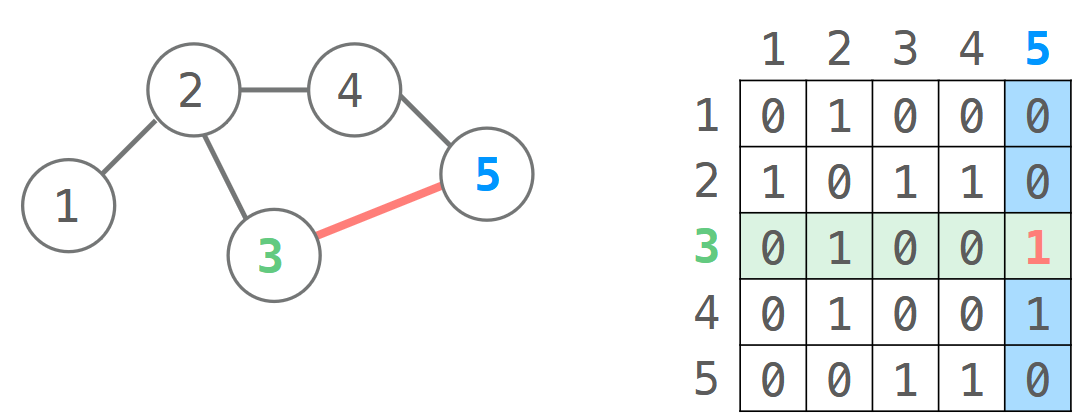
\includegraphics[width=0.5\textwidth]{Bilder/graph.png}
	\caption{Implementation eines Graphen in Java}
	\end{wrapfigure}
	\subsubsection{Java}
	Java bietet keine spezifische Datenstruktur an um einen Graphen darzustellen, jedoch kann man mit einem zweidimensionalen Array einfach eine definieren. Diese Datenstruktur nennt man Adjazenzmatrix oder Nachbarschaftsmatrix: \texttt{int Adjazenz [][]}. Dabei sind jeweils zwei Elemente miteinander anhand ihres Indexwertes verbunden. Elemente können entweder eine 1 oder eine 0 als Wert haben und diese sind dann in dieser Position mit dem anderen Element anhand ihres Indexes verbunden.
	\subsection{Baum}
	Ein Baum (oder Tree) ist eine speziellere Art von Graph wo keine Zylken enthalten sein können. Also darf ein Element nur nach unten aber nicht nach oben oder zur Seite verbunden sein. Das oberste Element eines Baumes nennt man dabei die Wurzel (root). Außer der Wurzel hat jedes Element einen Vorfahren, also ein Element das auf einer höheren Ebene liegt. Ein Vorfahre kann dabei beliebig viele Nachfolger haben. Elemente welche auf der selben Ebene liegen nennt man Geschiwster. Ein Element das nicht die Wurzel ist mit mindestens einem Nachfolger nennt man einen inneren Knoten und ein Element ohne Nachfolger nennt man Blätter. Für jeden Baum kann man auch einen Teilbaum definieren. Hierbei wird ein innerer Knoten als Wurzel eines neuen Baums definiert. Jeder innere Knoten in einem Baum kann als Teilbaum definiert werden. Ein Baum hat stets eine gewisse Menge an Ebenen, wobei die Wurzel auf der nullten Ebene (Ebene 0) ist. Jeder Nachfolger ist danach in einer weiteren Ebene.
	\subsubsection{Binärbaum}
	Ein Binärbaum ist eine spezielle Art von Baumstruktur. Hierbei darf jedes Element eines Baumes maximal zwei Kinder besitzen. Binärbäume sind in der Programmierung sehr nützlich da man viele Algorithmen effizient damit implementieren kann.
	\begin{wrapfigure}{l}{0.5\textwidth}
	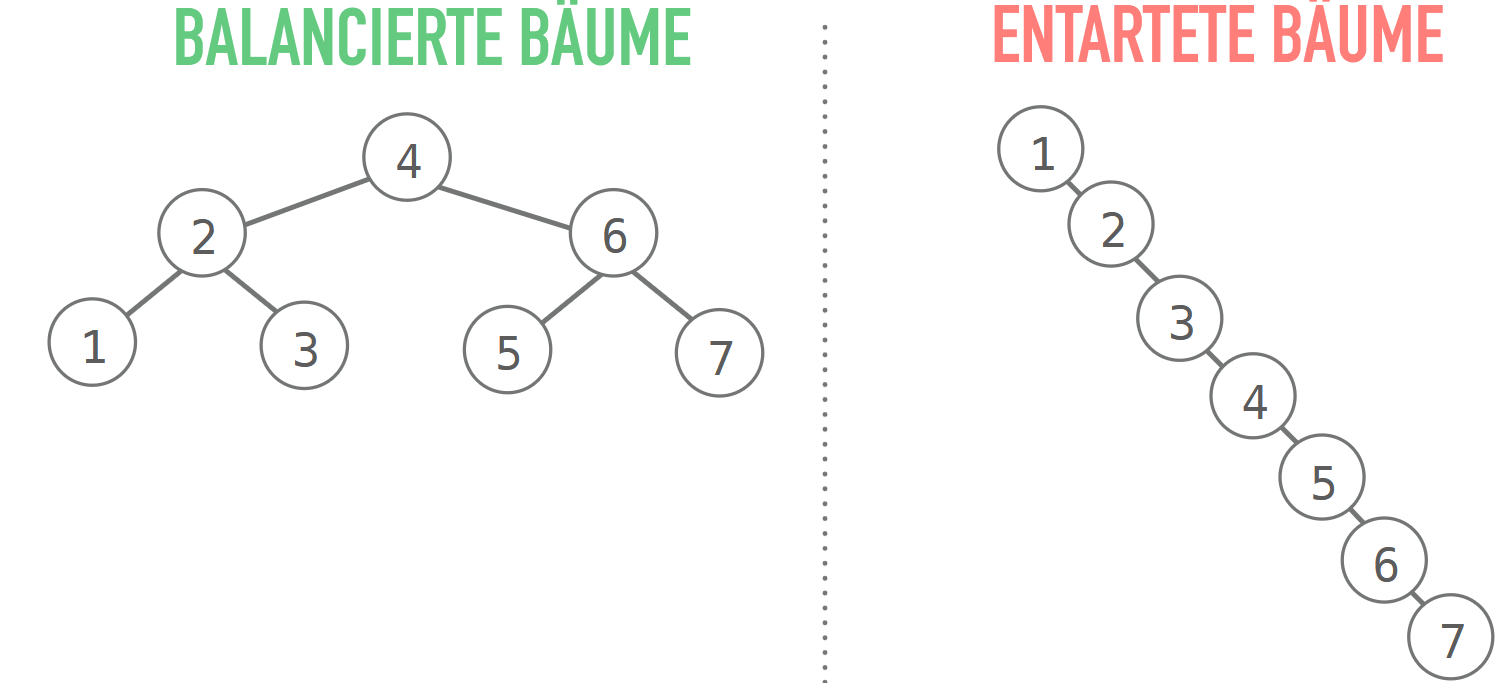
\includegraphics[width=0.5\textwidth]{Bilder/balanced.png}
	\caption{Jeweils ein balancierter und ein entarteter Baum}
	\end{wrapfigure}
	\subsubsection{Balancierte und Entartete Bäume}
	Bäume können zusätzlich balanciert oder entartet (oder keines von beiden) sein. Ein balancierter baum hat abhängig der Wurzel eine balancierte Menge an Elementen. So darf sich die Menge an Elementen nur um 1 unterscheiden. (Also kann ein balancierter Baum auf einer Seite 4 und auf der anderen Seite 5 Elemente haben.) Ein entarteter Baum ist das Gegenstück zu einem balancierten Baum wobei jeder Knoten nur maximal einen weiteren Knoten hat. So ist ein entarteter Baum wiederum eine Linked List und kann in einem Durchgang durchlaufen werden.
	\subsubsection{Java}
	Java hat auch keine Implementation von Bäumen jedoch ist dieser wiederum relativ einfach zu implementieren. So kann man ein eigenes 'Node' Objekt definieren und dessen Kinder in eine ArrayList speichern. Da man nur einen Elternteil haben kann, kann man diesen als einzelnes Nodeelement abspeichern. So verweist jedes Node Element auf dessen Kinder und auf dessen Elternteil und man kann den Baum durchlaufen.
	\subsection{Tree Traversal}
	Man kann einen Baum auf mehreren Wegen durchsuchen. Zwei dieser Wege sind die Depth-First Search (DFS) und die Breadth-First Search (BFS).
	\subsubsection{Depth-First Search (DFS)}
	Bei der Depth-First Search wird das Blatt jeden Elements vor den inneren Knoten durchsucht. Das wird realisiert indem man stets die Kinder eines Knotens auf einen Stack legt und anhand des Stacks das nächste Element durchsucht. Wenn man so zum Beispiel bei der Wurzel beginnt, durchsucht man diesen und legt alle Kinder auf den Stack. Danach wird das erste Kind als neue Basis verwendet und dessen Kinder (falls vorhanden) wiederum auf den Stack gelegt. So wird zuerst nur eine Linie jedes Knotens durchlaufen bis man an dessen Ende kommt und untersucht danach erst die restlichen Knoten (welche wiederum in einer Linie verlaufen können).
	\section{Algorithmische Grundpinzipien}
	Einige grundlegende Prinzipien der Algorithmik sind Divide-and-Conquer sowie Backtracking.
	\subsection{Divide-and-Conquer}
	Teile und Herrsche lautet die Devise. Dabei wird ein großes Problem in kleinere Teilprobleme aufgespalten und diese danach einzeln betrachtet. Das hat den Vorteil, dass man einen großen komplexen Ablauf auf viele kleine einfacherer Abläufe reduzieren kann um das Problem lösbarer zu machen. Diese Methode findet sich in vielen Aspekten der Softwareentwicklung wieder; selbst bei dem Schreiben von Code ist es eine gute Idee eine große Aufgabe in kleinere Teilaufgaben zu teilen.
	\subsubsection{Rekursion}
	Ein Teil wo dieser Ansatz relevant wird ist die Rekursion. Dabei ruft sich eine Methode wiederholt mit neuen Parametern (idealerweise einem Teilproblem) selbst auf. Das läuft im Gegensatz zu iterativen Algorithmen, welche mit einer Schleife den selben Code wiederholt ausführen. Dabei muss man jedoch beachten, dass sich \textbf{jedes rekursive Problem in ein iteratives transformieren lassen kann und umgekehrt.} \\
	Eine Rekursive Aufgabe braucht jedenfalls eine Abbruchbedingung da sie sonst endlich weiterläuft und einen Stack Overflow auslöst. Dieser geschieht, da jede neue Methode erneut auf den Call Stack gelegt wird und, falls die Methode unendlich verläuft, diese sich anhäufen bis er voll ist. \\
	Rekursionen können Vorteile gegenüber iterativen Ansätzen bieten. Bei geeigneten Aufgabenstellungen ist die Implementation bedeutend einfacher und erlaubt eine einfacherer Analyse durch rekursive Zeitgleichungen. Durch den rekursiven Aufruf verbraucht es jedoch mehr Speicher da jeder Durchlauf im Stack gespeichert werden muss. Zusätzlich kann es einen geringen Overhead durch die Notwendigkeit neue Methodenaufrufe zu generieren. In der Regel sollten rekursive Ansätze nur verwendet werden, wenn die Problemformulierung auch rekursiv geschieht. Wenn man zum Beispiel die Fibonacci-Zahlen berechnen will, benötigt man stets die beiden letzten zwei Ergebnisse womit es sich für eine rekursive Implementation gut eignet. \\
	Rekursion findet bei dem Durchsuchen von Baumstrukturen sowie bei einigen Datentypen wie Linked Lists oder Trees Anwendung.
	\subsection{Backtracking}
	Backtracking beschreibt das Verhalten, bei dem man nach Antreffen einer Sackgasse umdreht und die nächste Entscheidung trifft. Ein Beispiel dafür ist das Durchlaufen eines Labyrinths. Dabei wird, jedes Mal wenn man eine Sackgasse findet, zurückgegangen und die nächste Abzweigung gewählt. Ein Softwareproblem ist das Damenproblem. Dabei muss auf dem Feld eines Schachbretts mit n Reihen in jeder Reihe eine Dame platziert werden, sodass diese mit ihren Bewegungsmöglichkeiten keine andere Dame erreichen kann. Diese Strategie ist besonders effektiv wenn eine partielle Lösung in vielen Weisen erweitert werden kann. Dabei wird in der Theorie ein Baum aller Möglichkeiten gespannt und dieser danach durchlaufen.
	\section{Sortieren}
	Sortieren ist der Vorgang Daten in einem Array in ein bestimmtes Format zu bringen. Das kann von einer Sortierung nach Zahlengröße bis zum Code eines Characters reichen. Sortierverfahren werden in ihrer Komplexität und Laufzeit eingeordnet:
	\begin{itemize}
		\item{Elementare Sortierverfahren}
		\begin{itemize}
			\item{Relative einfache Implementationen jedoch auch hohe Laufzeit (Oft O($n^2$))}
		\end{itemize}
		\item{Effizientere Sortierverfahren}
		\begin{itemize}
			\item{Komplexere Implementation jedoch bedeutend niedrigere Laufzeiten (Immer unter O($n^2$))}
		\end{itemize}
	\end{itemize}
	\subsection{Sortiervarianten}
	Es gibt vier Eigenschaften von Sortieralgorithmen:
	\begin{itemize}
		\item{In-Place}
		\begin{itemize}
			\item{Es wird kein zusätzlicher Speicher benötigt um den Vorgang durchzuführen. Wenn dies nicht der Fall ist, nennt man das Out-Of-Place}
		\end{itemize}
		\item{Stable}
		\begin{itemize}
			\item{Elemente mit gleichem Schlüssel haben im Array nach der Sortierung immer noch die gleiche Anordnung. (Wenn zwei Elemente den Wert 5 haben, kommt die 5 die davor zuerst war auch danach noch davor vor.)}
			\item{Stable Sorts sind wichtig, wenn man eine Liste von Elementen mehrmals sortieren will. Wenn man also zuerst nach Nach- und dann nach Vornamen sortiert, will man eventuell, dass auch nach der zweiten Sortierung alle Nachnamen noch gleich sortiert sind.}
		\end{itemize}
		\item{Adaptiv}
		\begin{itemize}
			\item{Der Sortiervorgang ist schneller, wenn das Array bereits teilweise oder komplett vorsortiert ist. (Was zum Beispiel bei Insertion Sort der Fall ist)}
		\end{itemize}
		\item{Worst-Case Optimal}
		\begin{itemize}
			\item{Unabhängig von der Vorsortierung, wird das Array in O($n\ \log n$) sortier.}
		\end{itemize}
	\end{itemize}

	\subsection{Elementare Verfahren}
	Elementare Sortierverfahren die besprochen werden sind Insertion Sort und Selection Sort.
	\subsubsection{Insertion Sort}
	Das Array wird von links nach rechts durchlaufen, wobei jedes Mal wenn rechts ein kleinerer Wert als links steht werden diese vertauscht. Danach wird das gerade getauschte kleinere Element erneut mit dessen linkem Element verglichen bis es größer ist. Nachdem der rechte Rand des Arrays erreicht ist, ist das Array sortiert. Insertion Sort ist sehr effizient wenn das Array relativ klein ist und es schon teilweise vorsortiert ist.
	\subsubsection{Selection Sort}
	Es wird innerhalb des Arrays jeweils das kleinste Element gesucht und festgehalten bei welchem Index das sortierte Array beginnt. Sobald das kleinste Element rechts des sortieren Arrays gefunden wurde, wird es mit dem ersten Element des Arrays getauscht und der Index des sortierten Arrays um 1 erhöht. Selection Sort ist praktisch wenn man wenig temporären Speicher zur Verfügung hat und Speicherzugriffe teuer sind da jeweils nur ein Wert getauscht wird.
	\subsection{Effizientere Sortierverfahren}
	\subsubsection{Merge Sort}
	Bei dem Merge Sort wird das Array jeweils in 2 gleich große Hälften geteilt bis diese nicht mehr teilbar sind. Danach werden die jetzt einzelnen Teilelemente anhand ihrer Größe sortiert und somit kombiniert. Diese größeren Elemente werden wiederum auf die gleiche Weise kombiniert bis das Ursprungsarray sortiert zum Vorschein kommt. Die Zeitkomplexität des Mergesort ist O($n \log n$). Das hängt damit zusammen, dass in jeder Ebene des Splittens und Mergens ein Aufwand von O(n) besteht. Da das Array jedes Mal halbiert wird, kann man es als Binärbaum darstellen und man weiß, dass ein Binärbaum mit n Elementen eine Höhe von $\log n$ hat. Deshalb kann man diese Teile kombinieren um zu O($n \log n$) zu kommen. \\
	Merge Sort hat durch die Menge an Splits mit dem Call Stack einen relativ großen Overhead. Aus diesem Grund passiert es manchmal, dass Merge Sort mit Insertion Sort verbunden wird. Dabei wird das Array zuerst mit Mergesort gespalten wonach ab einer gewissen Mindestgröße (Oft 10 Elemente) die gespaltenen Arrays mit Insertion Sort sortiert werden.
	\subsubsection{Quick Sort}
	Quicksort funktioniert ähnlich zu dem Merge Sort, dass das Array bei jeder Iteration halbiert wird. Der Ablauf ist wie folgt:
	\begin{enumerate}
		\item{Das erste Element des Arrays wird als Pivot Element gewählt (Es gibt auch andere Strategien den Pivot zu wählen)}
		\item{Die Elemente des Arrays werden jeweils von links und rechts zur Mitte durchlaufen. Falls ein Element links des Pivot größer als dessen Wert und ein Element rechts des Pivot kleiner als dessen Wert ist, werden diese vertauscht, sodass jeweils kleinere und größere Werte links und rechts des Pivot stehen.}
		\item{In den Teilelementen wird das erste Element wiederum als Pivot gewählt und der Vorgang wiederholt.}
		\item{Sobald alle Teilelemente alleine stehen, ist das Array sortiert.}
	\end{enumerate}
	In diesem Fall wird der Pivot stets als das erste Element gewählt (was eine fragwürdige Wahl ist) und die Laufzeit im Worst Case hängt stark von diesem Faktor ab. Wenn ein zufälliges Pivotelement gewählt wird, ist die Laufzeit weniger abhängig von der Sortiertheit des Arrays.
	\subsection{Zusammenfassung}
	\begin{tabular}{| c | c | c | c | c | c | c |}
		\toprule
		&In-Place & Stabil & Adaptiv & Best Case & Avg. Case & Worst Case \\ \midrule
		Insertion Sort & \checkmark & \checkmark & \checkmark & O(n) & O($n^2$) & O($n^2$) \\ \hline
		Selection Sort & \checkmark & x & x & O($n^2$) & O($n^2$) & O($n^2$) \\ \hline
		Merge Sort & x & \checkmark & x & O($n \log n$) & O($n \log n$) & O($n \log n$) \\ \hline
		Quick Sort & \checkmark & x & x & O($n \log n$) & O($n \log n$) & O($n^2$) \\
		\bottomrule
	\end{tabular} \\
	\begin{itemize}
		\item{\textbf{Insertion Sort} ist sowohl in-place, als auch stabil und adaptiv.}
		\item{\textbf{Selection Sort} ist nicht in-place weil die Reihenfolge geändert werden kann und  nicht Adaptiv, da stets für jedes n das Array 1 Mal durchgangen werden muss.}
		\item{\textbf{Merge Sort} ist nicht in-place, da es zwei Hilfsarrays zum mergen benötigt und nicht adaptiv, da es immer die gleiche Laufzeit hat.}
		\item{\textbf{Quick Sort} ist in der genannten Ausführung nicht stabil (Kann es jedoch sein) und nicht adaptiv da er schlechter abschneidet, wenn das Feld sortiert ist.}
	\end{itemize}
		\section{Heap}
	Ein Heap ist eine spezielle Datenstruktur, welche anhand eines Binärbaums Elemente mit einer Priorität anordnet. Diese Priorität wird anhand einer Priority Queue wiedergegeben. Diese ist eine Warteschlange, welche anhand eines bestimmten Schlüssels sortiert ist. Die Queue selbst kann man nur manipulieren indem man das minimale oder maximale Element (Das Erste oder Letzte) entfernt. Jedes Mal, wenn ein Element in die Queue eingefügt wird muss dieses danach wieder in die richtige Form gebracht werden, wodurch die Komplexität der Operation O(n) ist. Auch wenn das Entfernen eine konstante Laufzeit hat, ist es unpraktisch, dass das Einfügen relativ ineffizient ist. Das Ziel wäre deshalb, dass alle Operationen auf die Priority Queue eine Komplexität von O(log(n)) haben.
	\subsection{Haldenbedingung}
	\begin{figure}[H]
	\centering
	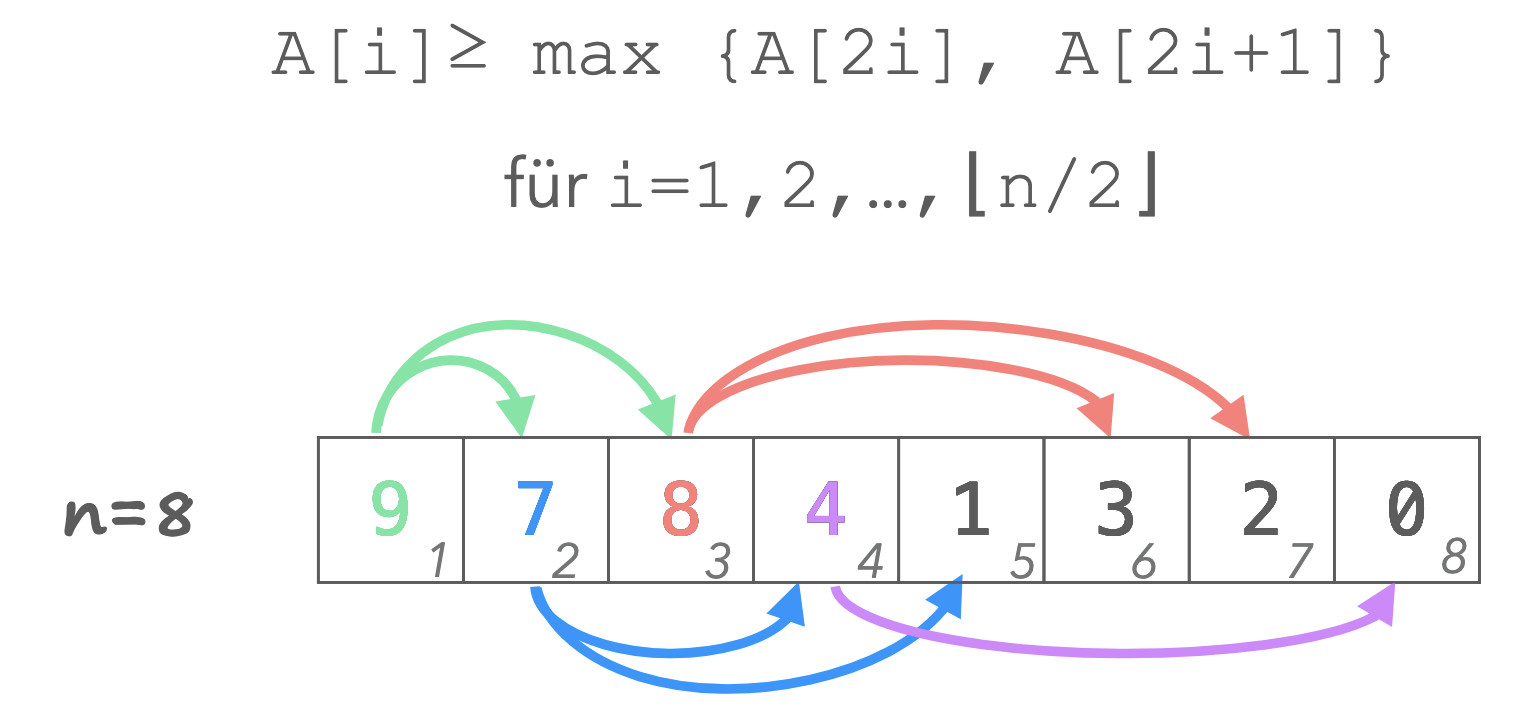
\includegraphics{Bilder/heap.png}
	\caption{Arrayrepräsentation eines Heaps}
	\end{figure}
	Das wird erreicht mittels Heap (Halde im Deutschen). Grundlegend zu dieser Datenstruktur ist die Haldenbedingung. Diese besagt, dass $A[i]\geq max \{A[2i], A[2i+1]\}$ oder ausgeschrieben, dass jedes Element an der Position i, größer sein muss als das Element an der Position $2i$ und $2i+1$. Das bedeutet wiederum, dass das größte Element des Heaps an erster Stelle stehen muss. Da jeweils der doppelte Index und dessen Inkrement abhängig von einem früheren Element sind, ist es in einer Binärbraumrepräsentation stets gegeben, dass der oberste Knoten (Das erste Element) der höchste Wert ist und jedes Kind jedes Knotens einen niedrigeren Wert hat als dessen Parent. Wenn diese Vorraussetzung gegeben ist, kann man sicher sein, dass man das höchste Element des Arrays an dessen erstem Index findet. Zusätzlich sind gewisse Suchvorgänge in konstanter Zeit möglich:
	\begin{itemize}
		\item{Parent eines Elements finden:}
		\begin{itemize}
			\item{$A[floor(Child\ Index\/2)]$}
		\end{itemize}
		\item{Linkes Kind finden:}
		\begin{itemize}
			\item{$A[Parent\ Index*2]$}
		\end{itemize}
		\item{Rechtes Kind finden:}
		\begin{itemize}
			\item{$A[Parent\ Index*2+1]$}
		\end{itemize}
	\end{itemize}
	\subsection{Heapify}
	Wenn ein Array die Haldenbedingung nicht erfüllt, kann man die Funktion Heapify verwenden um dieses in einen Heap zu verwandeln. Vorraussetzung dafür ist, dass alle darunterliegenden Teilbäume die Haldenbedingung erfüllen (Jedes Kind ist kleiner oder gleich des Parents). Dabei wird für jedes Teilelement der Parent und dessen Kinder verglichen und diese vertauscht, falls der Parent nicht das größte Element ist. Dadurch kann zwar die Haldenbedingung verletzt werden, das getauschte Element sickert jedoch weiter, wodurch die Vorraussetzung wieder erfüllt wird.
	\subsection{\texorpdfstring{Build\_Heap}{Build Heap}}
	Zusätzlich zu Heapify existiert auch die Build\_Heap Funktion, welche aus einem unsortierten Array einen Heap erstellt. Dabei arbeitet es von unten nach oben um jeden Teilbaum des Heaps in einen Heap zu verwandeln. Da ein Knoten ohne Kinder ein Heap ist, erfüllen alle Blätter des Baumes bereits die Haldenbedingung, wodurch man von dort beginnen kann.
	\subsection{Heap Sort}
	Der Heap Sort bedient sich der Eigenschaft eines Heaps, dass das größte Element stets an erster Stelle steht. Das passiert nach einem festen Schema:
	\begin{enumerate}
		\item{Ein unsortiertes Array wird verhaldet}
		\item{Das erste Element wird mit der letzten Stelle vertauscht}
		\item{Die Länge des Arrays wird um 1 verringert}
		\item{Falls das getauschte Element die Haldenbedingung verletzt, muss Heapify aufgerufen werden}
	\end{enumerate}
	\section{Radix Sort}
	Bis jetzt verwendeten Sortierverfahren stets nur algorithmische Operatoren um Elemente miteinander zu vergleichen. Radix Sort ist jedoch ein nicht-vergleichender Sortieralgorithmus bei welcher jedem Element anhand seines Inhalts ein Fach zugewiesen wird (Ähnlich zu einem Hashingalgorithmus). Dabei wird für jede Stelle des Ergebnisses dieses in sich sortiert. Radix arbeitet dabei stets in zwei Phasen: Der Streu- und der Sammelphase. In der Streuphase werden alle Elemente anhand des Kriteriums in die Fäche gelegt. Bei der Sammelphase werden danach diese Fäche in umgekehrter Reihenfolge wieder angeordnet. Elemente werden also von der kleinsten zur größten Zahl vom ersten Element im Fach zum letzten Element angeordnet. Das führt dazu, dass die Sortireung innerhalb eines Faches zwischen Phasen erhalten bleibt. \\
	Die Laufzeit des Radix Sort hängt von der Menge an Elementen sowie der Menge an Stellen im längsten Element ab, da die Landau Notation jedoch Konstanten ignoriert, ist die Laufzeit stets O(n), was diesen Sortieralgorithmus zu einem der effizientesten macht.
	\section{Suche}
	Nachdem ein Array sortiert wurde, kann man es durchsuchen. Eine Suche hat dabei ein spezifisches Ziel, welches gefunden werden will. Anders als die Sortierung kann eine Suche fehlschlagen, wodurch der worst case eintritt (Das gesamte Array muss durchsucht werden, es wurde jedoch kein Ergebnis gefunden.).
	\subsection{Sequentielle Suche}
	Eine Liste kann natürlich auch durchsucht werden, wenn sie nicht sortiert ist, man muss dabei jedoch auf die primitivste Methode des Suchens zurückgreifen: Der Sequentiellen Suche in der jedes Element von vorne nach hinten angesehen wird, um das gesuchte zu finden. Im besten Fall ist das gesuchte Element an der ersten Stelle, wodurch die Komplexität O(1) beträgt. Im schlechtesten Fall ist das Element an letzter Stelle oder nicht vorhanden, wodurch das gesamte Array durchsucht werden muss.
	\subsection{Binärsuche}
	Die Binärsuche ist der erste 'nicht-triviale' Suchalgorithmus und kann nur auf vorsortierte Arrays angewandt werden. Dabei wird jeweils der Wert in der Hälfte des Index' des Arrays angesehen und anhand dessen in der rechten oder linken Seite weitergesucht. Wenn der Wert geringer ist, sucht man links und wenn der Wert rechts ist sucht man rechts. Da man so bei jedem Schritt die Länge des noch zu durchsuchenden Arrays halbiert, hat man maximal log n Schritte (Da es als Binärbaum gespannt werden kann), was auch den worst case darstellt. Im Best Case ist das Element wiederum genau in der Hälfte des Arrays und wird sofort angetroffen.
	\subsection{Interpolationssuche}
	Die Interpolationssuche versucht eine Schätzung anhand der Werte des Arrays zu machen um anhand dessen im Array nachzusehen. Dabei wird die Menge der Elemente sowie die Werte am Anfang und Ende des Arrays in Betracht gezogen. Das passiert anhand dieser Formel: $t=from+\lfloor(to-from)*\frac{x-A[from]}{A[to]-A[from]}\rfloor$. Die Effizienz dieses Suchalgorithmus' hängt von der Verteilung der Werte ab. Falls die Werte perfekt gleichverteilt sind, findet die Interpolationssuche einen Wert im ersten Schritt. Falls die Werte jedoch einen exponentiellen Anstieg haben, muss das gesamte Array wie in der sequentiellen Suche durchsucht werden.
	\subsection{Quadratische Binärsuche}
	Bei der quadratischen Binärsuche wird der gleiche Vorgang wie in der Interpolationssuche mit einer verkürzten Folgesuche kombiniert. Der erste Wert wird mittels Interpolationssuche gefunden und anhand dessen entschieden ob links oder rechts des Werts weitergesucht werden soll. Danach wird jedoch nicht eine weitere Interpolationssuche ausgeführt und stattdessen in Schritten welche der Wurzel der Länge des zu durchsuchenden Arrays entsprechen. Falls das Array also 10 Werte hat, würde ein Sprung 3 Zeilen groß sein, da $\lfloor\sqrt{10}\rfloor=3$. Nach jedem Sprung wird danach überprüft ob der Wert jetzt größer oder kleiner ist und nimmt diese Sprunggröße als das neue Array. Da das Array mit $\sqrt{n}$ Sprüngen durchlaufen werden kann, hat es im worst case auch eine Laufzeit von O($\sqrt{n}$) (Was jedoch schlechter ist als O(log n)) \\ \\
	\begin{tabular}{| l | l | l | l | l |}
		\toprule
		Algorithmus & Best Case & Worst Case \\ \midrule
		Sequentielle Suche & O(1) & O(n) \\ \hline
		Binärsuche & O(1) & O(log n) \\ \hline
		Interpolationssuche & O(1) & O(n) \\ \hline
		Quadratische Binärsuche & O(1) & O$\sqrt{n}$ \\
		\bottomrule
	\end{tabular}
	\section{Hashing}
	Hashing ist der Prozess ein Element mithilfe einer verlustbehafteten Kodierung zu einem anderen Wert zu konvertieren. Dieser Vorgang löst das sogenannte Wörterbuchproblem, welches das Einfügen, Löschen und Lesen von Key-Value Paaren gespeicherten effizient lösen soll. \\
	Ein Hash verwendet eine Hashing Funktion um den Speicherplatz des Elements zuzuweisen. Durch Anwenden der Funktion kann ein Element danach effizient wiedergefunden werden. 
	\subsection{Kollision}
	Hashingfunktionen sind nicht injektiv, weshalb unterschiedliche Werte zum gleichen Hashwert führen kann. In diesem Fall führt das zu einer Kollision und muss entsprechend gehandhabt werden. Im Idealfall hat eine Hash Table eine Komplexität von O(1) für alle Operationen. Das wird jedoch verlangsamt, wenn Kollisionen in der Hash Tabelle dazu führen, dass das Ziel erneut durchsucht werden muss. Die Wahrscheinlichkeit einer Kollision ist abhängig vom Load Factor $\alpha$, welcher die Menge der Elemente n geteilt durch die Menge der Plätze in der Tabelle m ist: $\alpha=\frac{n}{m}$.
	\subsection{Operationen}
	Eine Hash Table hat vier elementare Operationen: \textit{put, get, contains} und \textit{remove}:
	\begin{itemize}
		\item{put}
		\begin{itemize}
			\item{Fügt ein Element der Tabelle hinzu}
		\end{itemize}
		\item{get}
		\begin{itemize}
			\item{Sucht ein Element in der Tabelle}
		\end{itemize}
		\item{contains}
		\begin{itemize}
			\item{Überprüft ob ein Element in der Tabelle existiert}
		\end{itemize}
		\item{remove}
		\begin{itemize}
			\item{Entfernt ein Element aus der Tabelle, falls vorhanden}
		\end{itemize}
	\end{itemize}
	Jede dieser Operationen benötigt die Hash Funktion, weshalb sie so effizient wie möglich sein sollte.
	\subsection{Hashfunktion}
	Die Hashfunktion ist das Herz der Hashtable, da sie die Werte Elemente in die finalen Werte überträgt. Eine Hashfunktion sollte idealerweise zu gleichverteilten Werten führen um so Kollisionen zu vermeiden und alle möglichen Indizes ansprechen können, da man sonst Speicherplatz und Effizienz verschwenden würde. Ähnliche Werte sollten auch möglichst gut getrennt sein, damit die Daten nicht auf den Hashwert zurückführbar sind. Es sollte auch unabhängig von Mustern in den Daten sein um weiter Kollisionen zu vermeiden.
	\subsubsection{Divisionsmethode}
	Ein einfacher Weg eine Hashfunktion zu implementieren, ist den Wert durch eine Zahl zu teilen und den Rest als Wert zu verwenden. Diese Werte sind sehr schnell berechenbar, können jedoch leicht zu Kollisionen führen, da abhängig von dem gewählten Wert nahe beieinander liegende Werte auch zum selben Hashwert führen würden.
	\subsubsection{Multiplikationsmethode}
	Eine Alternative ist es den Wert mit einem bestimmten Wert zu multiplizieren und diesen danach zu dividieren um den Rest zu nehmen, zum Beispiel nach der Formel: $h(k)=\lfloor m\times(k\times A mod 1)$, wobei A der zufällige Wert ist. Ein guter Wert zur Wahl von A kann $\frac{\sqrt{5}-1}{2}=0.6180339887$, was der Goldene Schnitt ist.
	\subsubsection{Horner's Methode}
	Zum Hashing von Strings kann man Horner's Methode anwenden, bei der Strings jeweils als große Zahlen anhand ihres numerischen Werts behandelt werden. Diese werden jeweils mit einem fixen Wert multipliziert (Am besten eine relativ kleine Primzahl wie 31) und zum Endergebnis addiert. Dieses Ergebnis wird dann auf die gleiche Weise dividiert.
	\subsection{Kollisionen}
	Bei Kollisionen gibt es zwei gängige Methoden diese zu behandeln: Mit Überlauflisten oder per offener Adressierung.
	\subsubsection{Überlaufliste}
	Überlauflisten sind Listen, welche an den Destinationen der Hashtabelle stehen. Wenn es zu einer Kollision kommen würde, wird der Wert stattdessen zu einer Liste ausgelagert. Sobald wieder nach diesem Wert gesucht wird, werden danach alle Listen dieses Buckets durchsucht. \\
	Man muss dabei die Operationen der Hashtabelle verändern. Für \textit{put} muss man, falls das Ziel voll ist, eine neue Liste erzeugen und diese zwischen der ersten Liste und dem Ursprung setzen (Also ganz vorne einfügen und alles 1 nach hinten schieben.) \\
	Für \textit{remove} muss man nach Entfernen eines Wertes überprüfen ob die Liste noch Werte enthält und die vorangehende und folgende Liste miteinander verbinden. \\
	Vorteil dieser Strategie ist, dass theoretisch unendlich viele Werte pro Tabelle gespeichert werden können, es macht jedoch die Speicherverwaltung komplexer und benötigt mehr Speicherplatz, da man auch die Pointer speichern muss.
	\subsubsection{Offene Liste}
	Bei der offenen Liste wird stattdessen, falls eine Kollision geschehen würde, die nächste Zelle der Tabelle gewählt, bis eine freie angetroffen wird. Bei Verwendung einer offenen Liste wird zusätzlich zum Zielindex der Funktion noch die Probingnummer hinzugefügt, welche den Offset vom Index anhand der Versuche darstellt. Dieser Offset kann eine Maximalgröße von $m-1$ haben, da dann das gesamte Array durchlaufen wurde und es damit voll ist. Das ist auch einer der Nachteile der offenen Liste, da es trotzdem durch die Größe des Arrays limitiert ist. Dafür ist es jedoch bedeutend einfacher zu implementieren, da man einfach den nächsten freien Wert im Array nimmt.



	
	
	
	























	
\end{document}